\chapter{Methodology}
\label{ch:methodology}
The overall process of developing the WebArgo platform presented in this work consisted of the following steps:
\begin{enumerate}
  \item Theoretical design of the platforms Architecture
  \item Development of a Proof of Concept prototype
  \item Development process from the prototype to the WebArgo platform
  \begin{itemize}
    \item Implementation of \acs{API} and web interface
    \item Usage of generic job and task entities to support any kind of custom job
    \item Add WebAssembly Support for multiple programming languages
    \item Implement support for various output datatypes (primitiv datatypes, lists, files as binary)
  \end{itemize}
  \item Deployment of the web application
  \begin{itemize}
    \item Orchestrate all components of the WebArgo platform with Docker Compose \cite{conclusion:docker}
    \item Host the project on a cloud services (\emph{openstack} from h\_da)
    \item Implement user entity with specific user roles to enable security
    \item Implement security measures through authentication \& authorization
  \end{itemize}
  \item Enhance robustness of the platform
  \begin{itemize}
    \item Implement system recovery measures and persistence of critical data
    \item Adjust scheduling algorithm to ensure the completion of jobs, even when workers are unreliable
    \item Eliminate bugs through testing the application
  \end{itemize}
  \item Implement the visualization of the Mandelbrot set in multiple languages as the benchmark job
  \item Evaluation of the platform through multiple experiments 
\end{enumerate}
The following content of this chapter enumerates and describes all the technologies, frameworks, and tools utilized in the development of the WebArgo volunteer computing platform, along with the reasoning for their selection. The first section provides the framework selection for the three components of WebArgos architecture, as described in \autoref{sec:concept:architecture}. The following section describes each of the three key web technologies and corresponding tools utilized in the implementation of WebArgo to establish a foundation for the following \autoref{ch:implementation}, which focuses on the implementation. The last section of this chapter introduces the approach to benchmark WebArgo, which is used in \autoref{ch:evaluation} to evaluate the developed platform.

\section{Frameworks}
\label{sec:methodology:frameworks}
This section introduces the frameworks selected for the development of all components of the WebArgo platfrom. The following criteria were used to guide the selection of a suitable framework for the backend, frontend as well as the database:
\begin{itemize}
    \item The framework is well-tested and provides a stable \ac{LTS} version.
    \item The framework is popular among web developers.
\end{itemize}

\subsection{Backend}
\label{subsec:methodology:frameworks:backend}
It was crucial for the backend framework to be popular among web developers. Working with a popular framework improves the development process by ensuring the availability of detailed educational resources online as well as various online support forums. Additionally, a widely used framework increases the likelihood that the platform can be maintained or further extended by other programmers.
\begin{figure}[htbp]
 \centering
 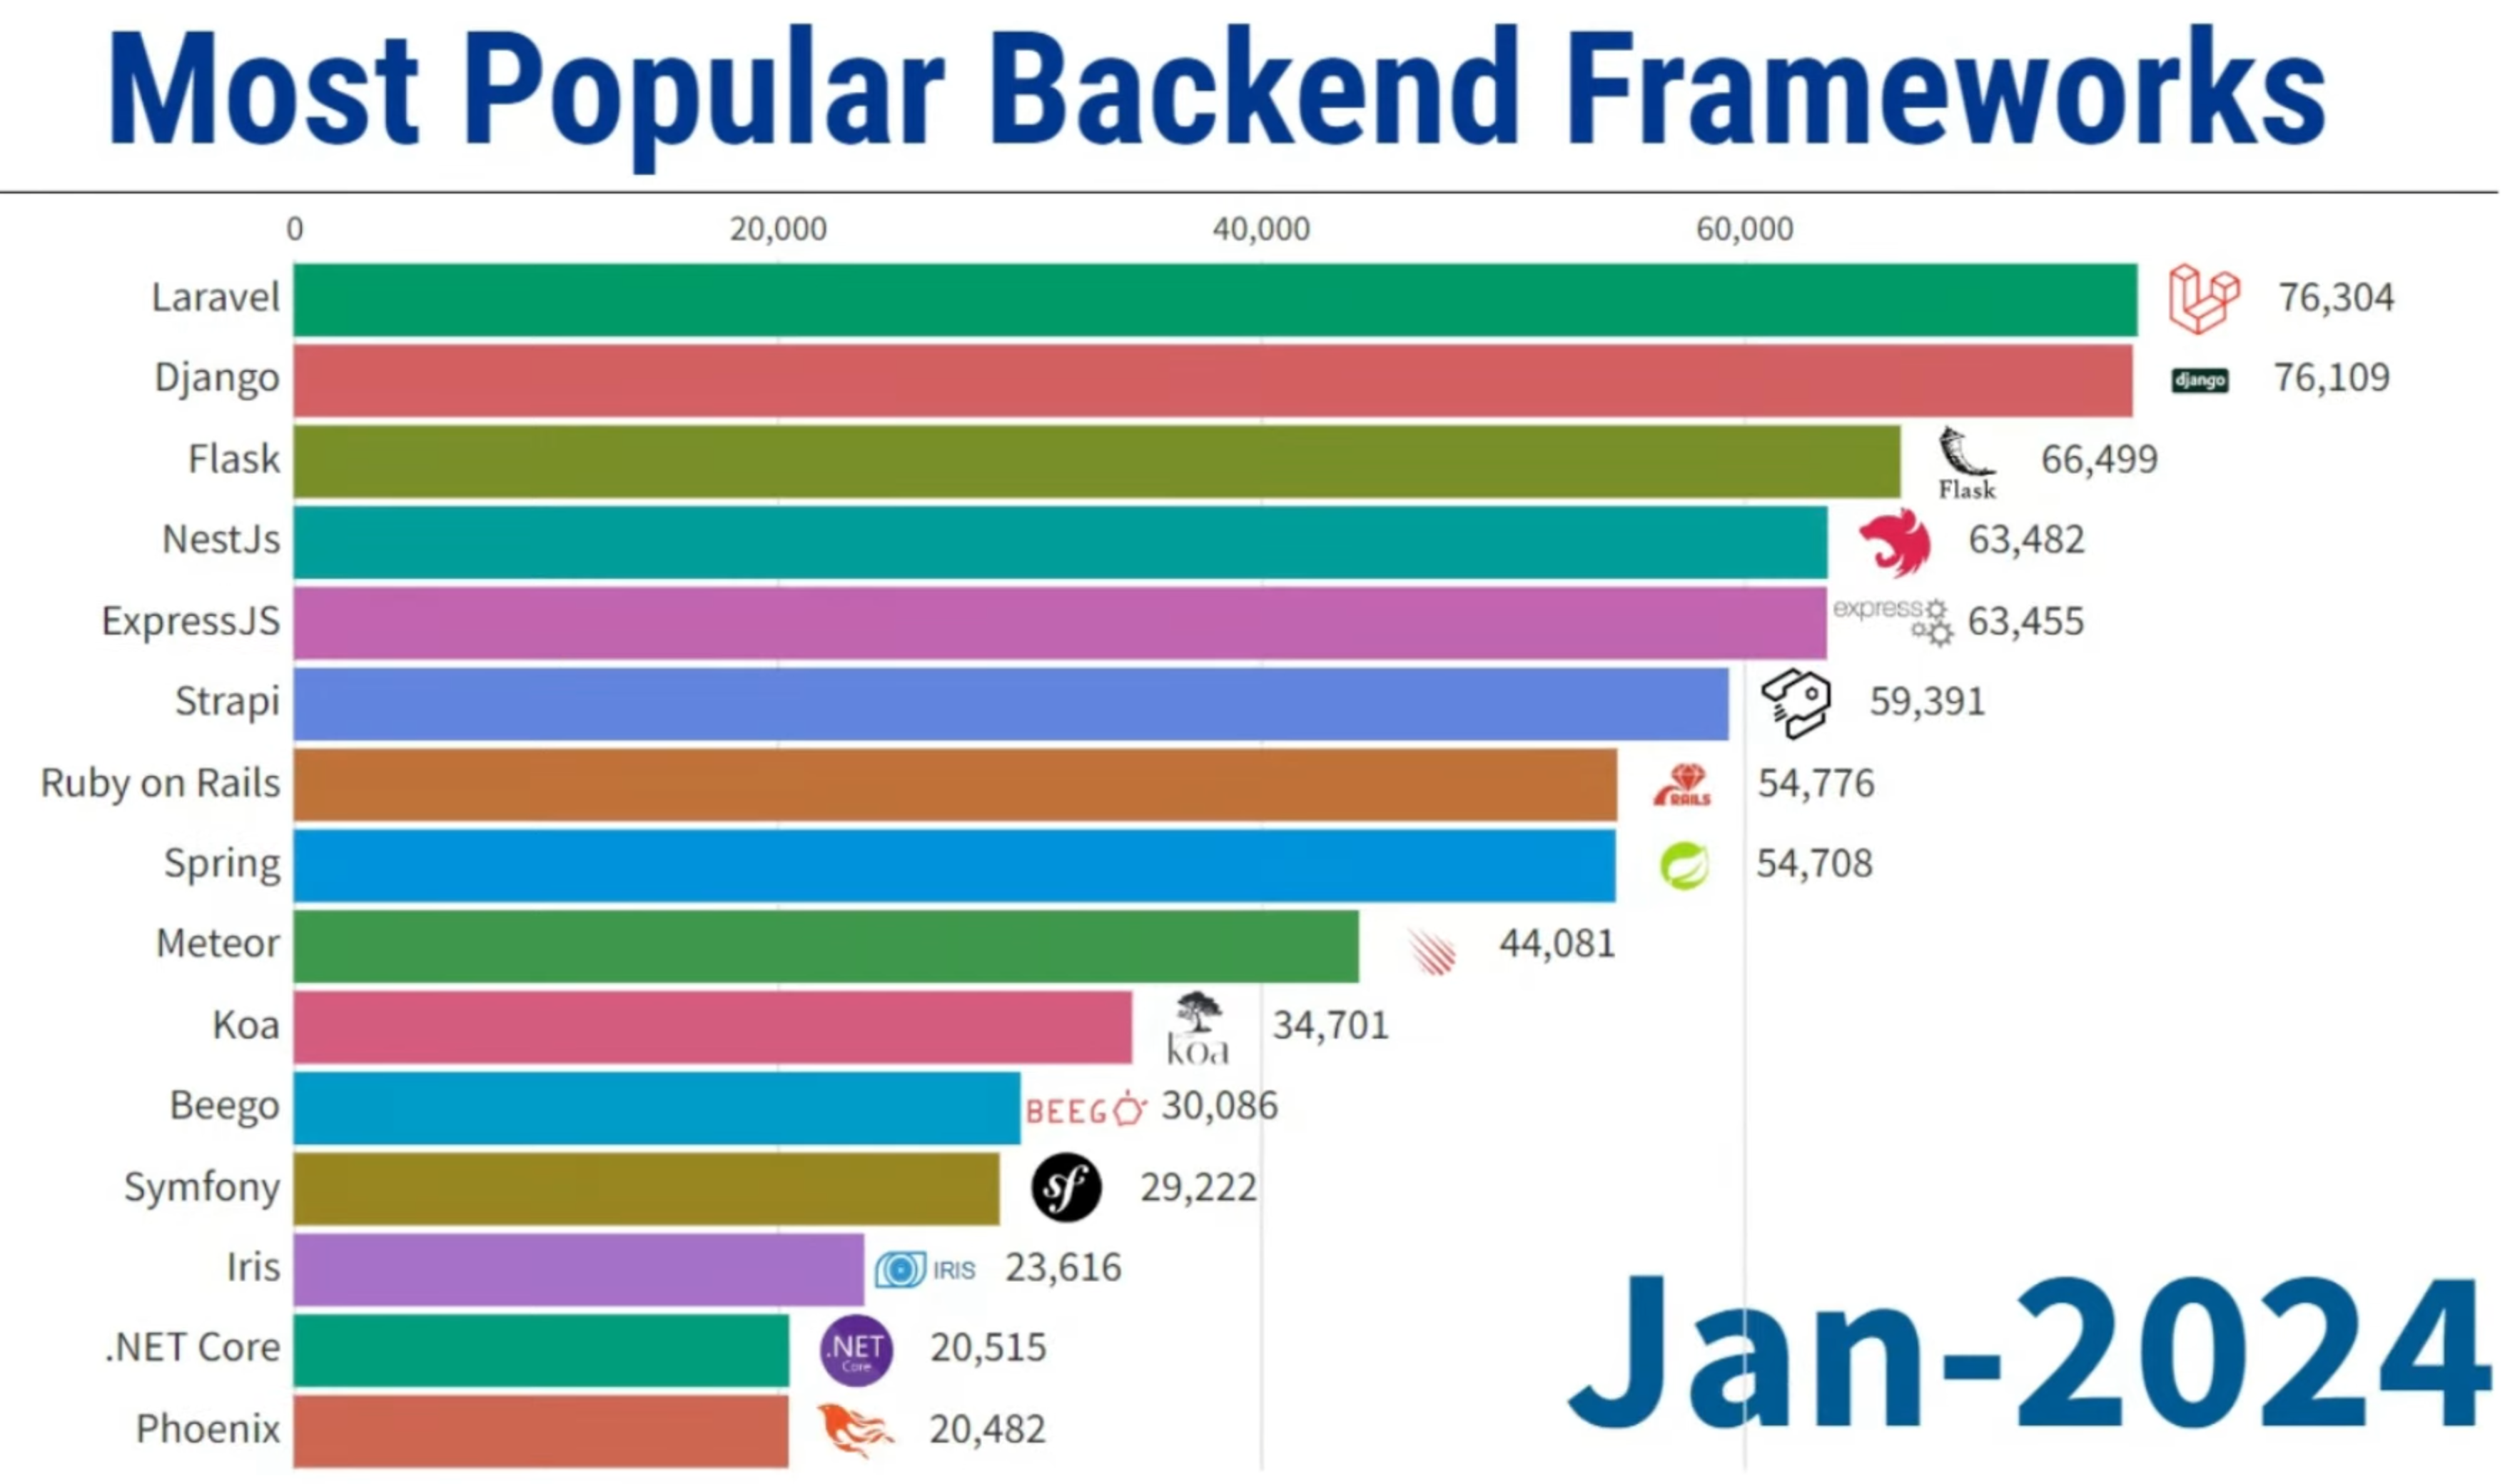
\includegraphics[width=0.95\textwidth]{gfx/figures/Popular_BE.png}
 \caption{Most Popular Backend Frameworks (Jan 2024) by GitHub Stars \cite{backend:popularity}}
 \label{fig:methodology:popularBE}
\end{figure}
~\\
The 15 most popular backend frameworks of January 2024 are displayed in \autoref{fig:methodology:popularBE}. The popularity for each framework of this list is calculated by the number of GitHub Stars from repositories listed in a GitHub Archive \cite{backend:popularity}. The selection options of the backend framework where based on this popularity list.

In addition to the previously stated criteria, the selected backend framework needed to meet specific performance requirements. It was essential for the framework to efficiently handle multiple connected clients with minimal latency. Furthermore, the framework's internal computation speed was critical, particularly for preparing input arguments for each task and managing task scheduling across all clients. The goal was to reduce overhead as much as possible to ensure high performance.
\begin{figure}[htbp]
  \myfloatalign
  \subfloat[Best fortunes responses per second (2023-10-17) \cite{backend:benchmark2}]{
    \label{fig:methodology:benchmark2BE}
    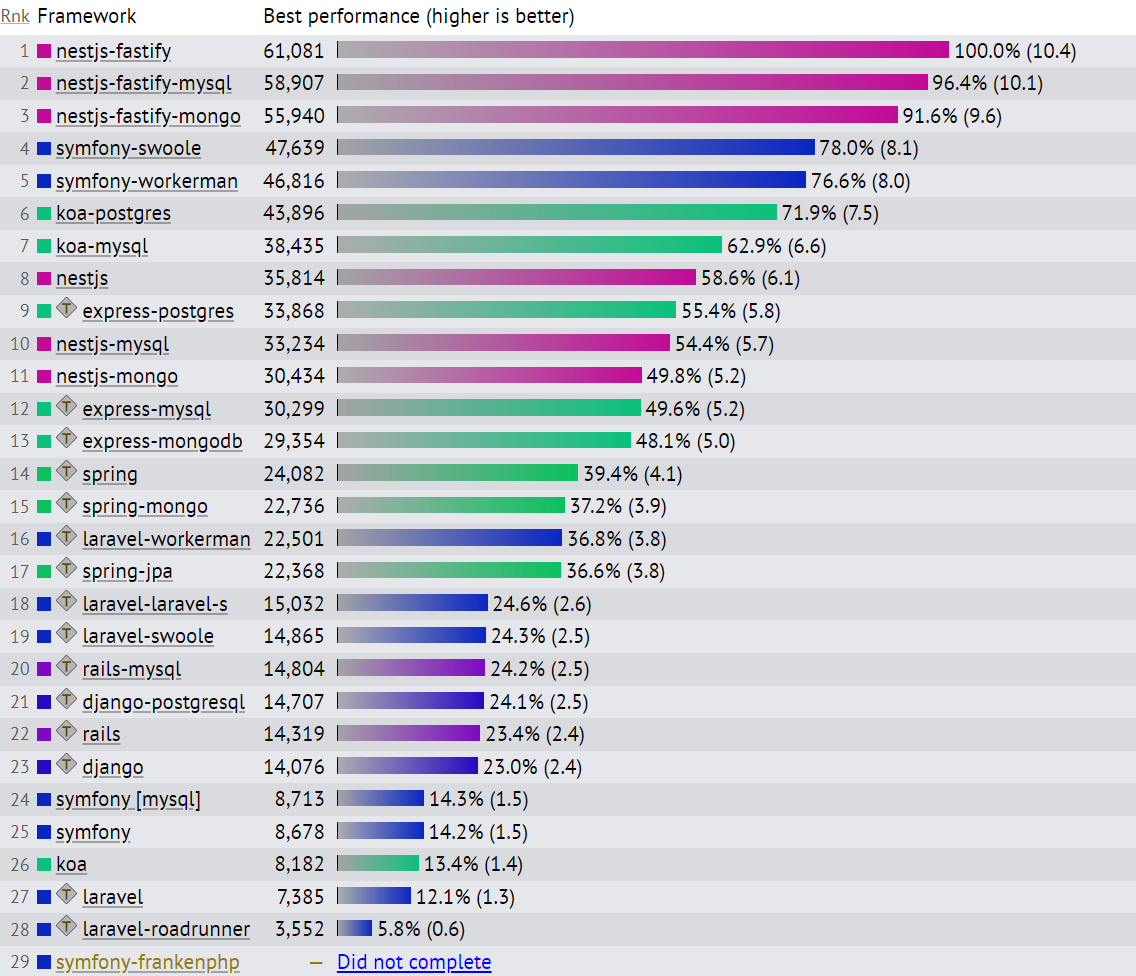
\includegraphics[width=.95\linewidth]{gfx/figures/Benchmark2_BE.png}
  }
  \caption{Most Popular Backend Frameworks from \autoref{fig:methodology:popularBE} Ranked by Performance.}
  \label{fig:methodology:benchmarkBE}
\end{figure}
~\\
To identify a high-performance framework, the most popular backend frameworks listed in \autoref{fig:methodology:popularBE} were compared by using two independent benchmark sources. The results of these benchmarks are presented in \autoref{fig:methodology:benchmarkBE}, where the frameworks are ranked from top to bottom based on their performance. It is important to note that some frameworks from the list in \autoref{fig:methodology:popularBE} where not part of these specific benchmarks. Both benchmark sources simulated numerous clients sending requests to each backend and measuring the number of successful responses per second in order to determine the performance \cite{backend:benchmark1, backend:benchmark2}.
\clearpage
\begin{figure}[htbp] \ContinuedFloat
  \myfloatalign
  \subfloat[Requests/Second (2024-06-25) \cite{backend:benchmark1}]{
     \label{fig:methodology:benchmark1BE}
     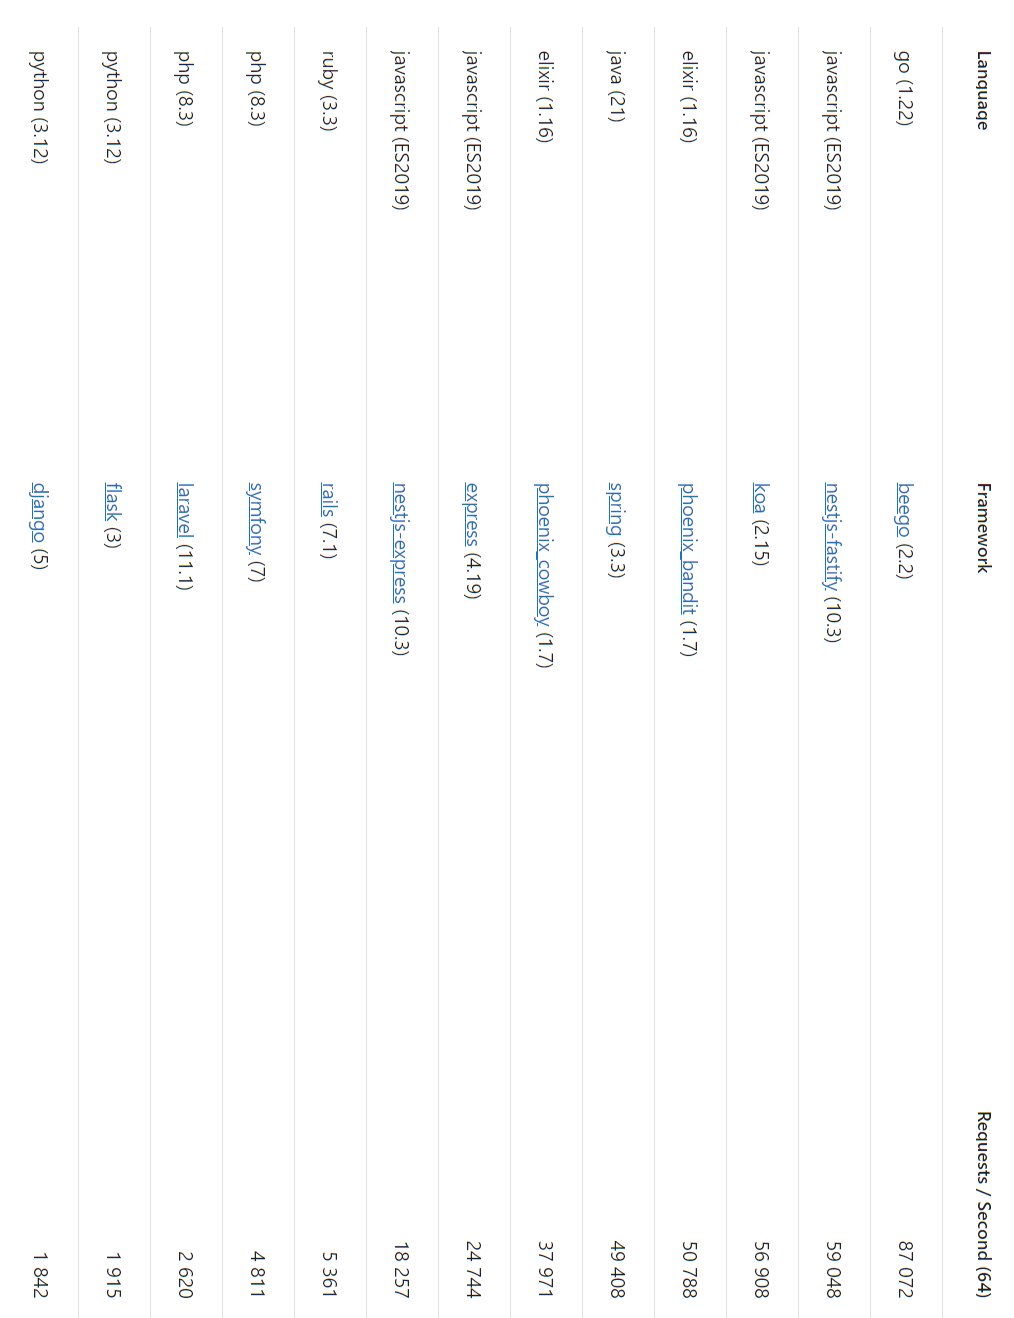
\includegraphics[width=.95\linewidth]{gfx/figures/Benchmark1_BE-smal.png}
   }
   \caption{Most Popular Backend Frameworks from \autoref{fig:methodology:popularBE} Ranked by Performance.}
   \label{fig:methodology:benchmarkBE}
\end{figure}
~\\
Finally, NestJS \cite{methodology:nestjs} with Fastify was selected as the backend framework. It performed exceptionally well in both benchmarks shown in \autoref{fig:methodology:benchmarkBE} and is also a popular choice among developers.
%\begin{figure}[htbp] \ContinuedFloat
%  \myfloatalign
%  \subfloat[Requests/Second (2024-06-25) \cite{backend:benchmark1}]{
%     \label{fig:methodology:benchmark1BE}
%     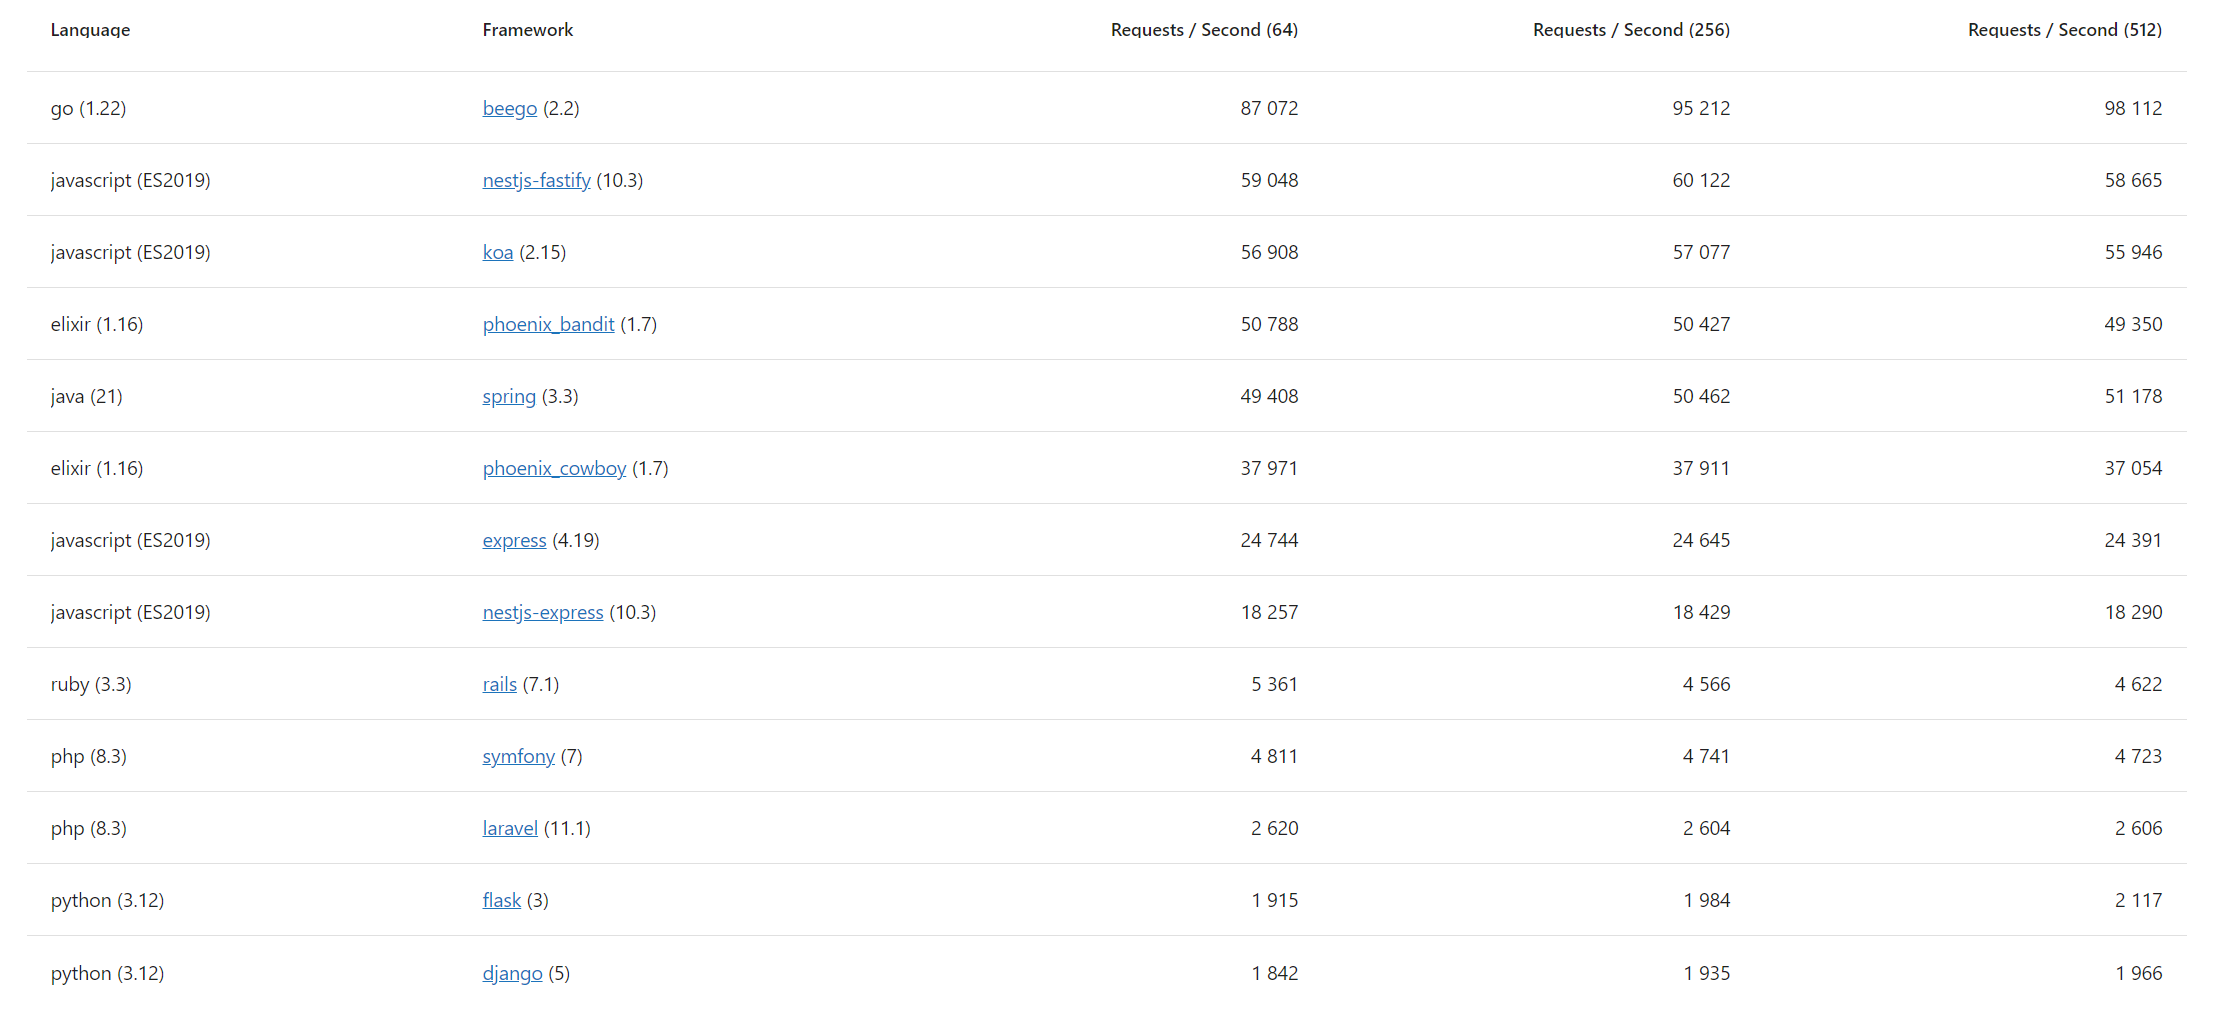
\includegraphics[width=.75\linewidth]{gfx/figures/Benchmark1_BE.png}
%   }
%   \caption{Most Popular Backend Frameworks from \autoref{fig:methodology:popularBE} Ranked by Performance.}
%   \label{fig:methodology:benchmarkBE}
%\end{figure}
\begin{figure}[htbp]
  \centering
  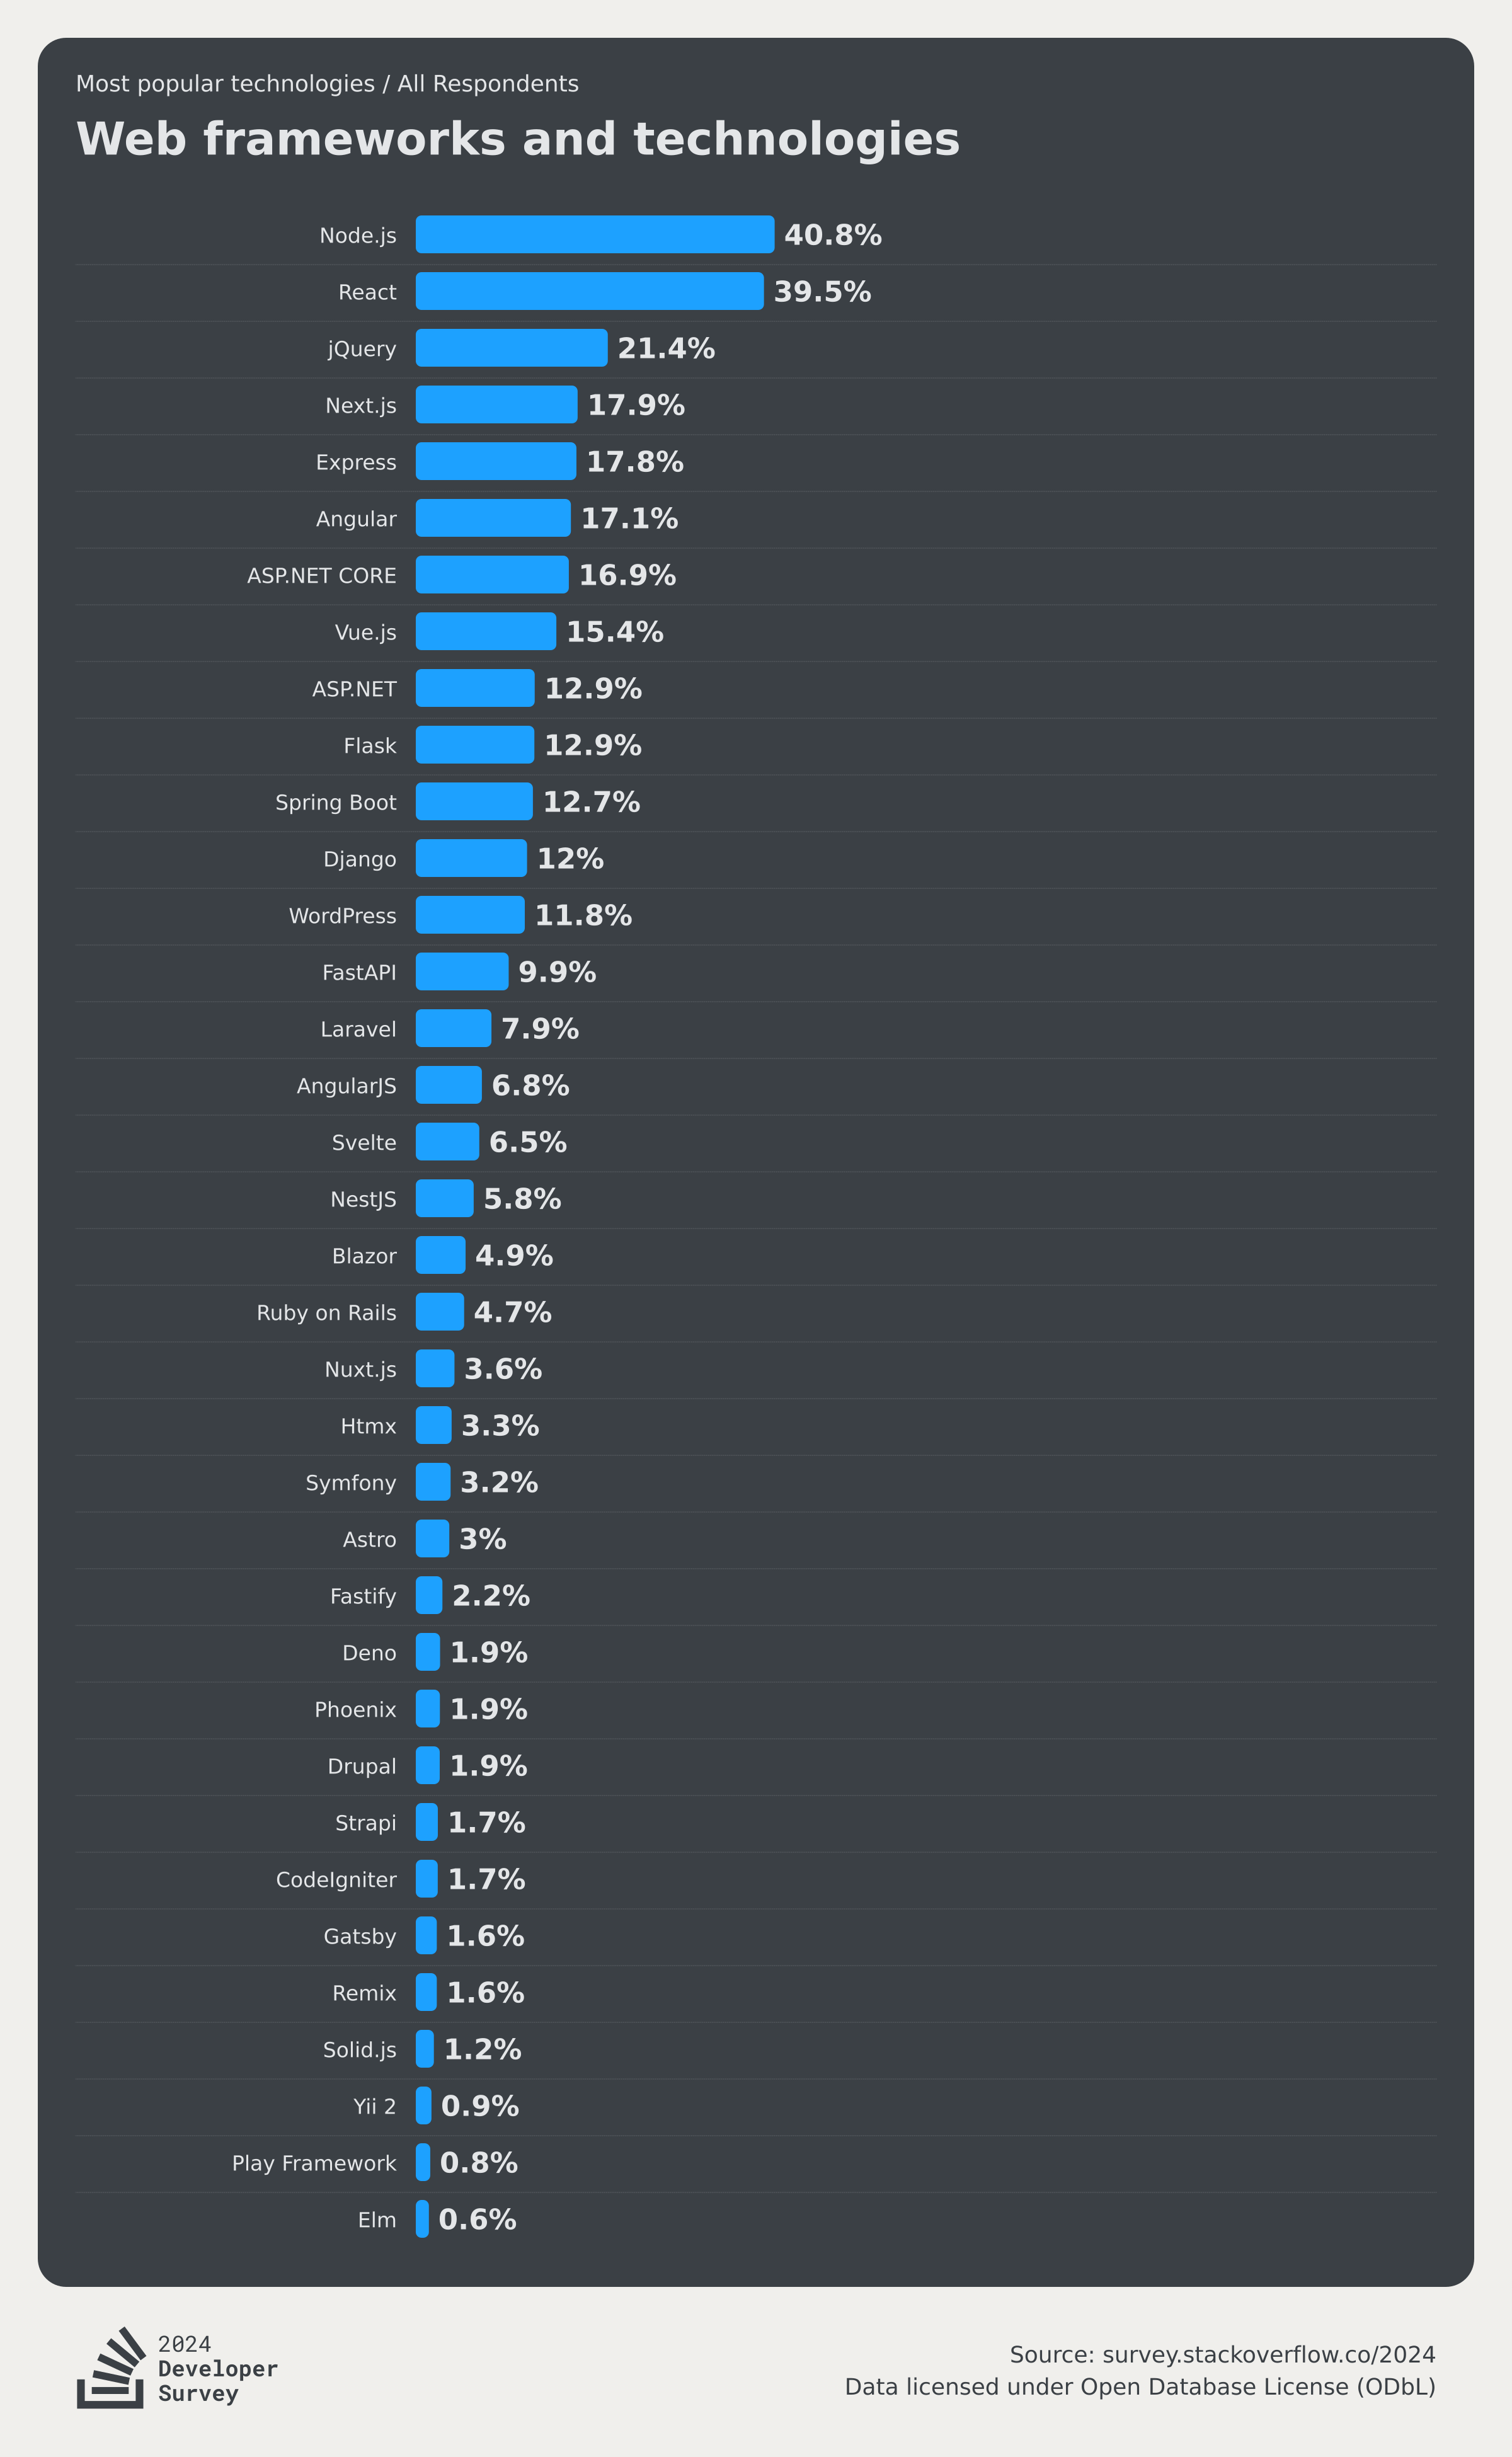
\includegraphics[width=0.95\textwidth]{gfx/figures/FrameworkSurvey2024.png}
  \caption{Most Used Web Frameworks and Technologies in 2024 (Developer Survey from Stack Overflow) \cite{frontend:popularity}}
  \label{fig:methodology:popularFE}
\end{figure}
\clearpage

\subsection{Frontend}
\label{subsec:methodology:frameworks:frontend}
The criteria stated in \autoref{sec:methodology:frameworks} also applied for the selection of a framework for the frontend. \autoref{fig:methodology:popularFE} shows the 36 most used frameworks among web developers in July 2024 \cite{frontend:popularity}. This statistic was collected by Stack Overflow and is the result of a survey. In this survey web developers have been asked which web frameworks and web technologies they had been working with in the past year, and which do they want to work in over the next year \cite{frontend:popularity}. The two most popular options are, by far, Node.js and React with each around 40\% of votes. While Node.js is mainly used for backend development React is a JavaScript library used for frontend development. This is qualifying React as the choice of technology for the frontend development. Ranking fourth in \autoref{sec:methodology:frameworks} is Next.js with 17.9\% of votes. Next.js is a web framework based on React \cite{methodology:nextjs} and according to the survey the most popular React web framework in the year 2024. Therefore Next.js was selected as the framework for frontend development.

\subsection{Database}
An object-relational database system was identified to fulfill the platform's requirements, as these systems typically offer high performance capabilities and the entities described in \autoref{sec:concept:terminology} can be represented with an object-relational database schema.

PostgreSQL is an open source object-relational database system that has been actively developed for more than 35 years \cite{methodology:db}. Therefore it has gained a strong reputation for reliability, feature robustness, and performance \cite{methodology:db}, hence PostgreSQL was selected as the database management system for this implementation.

\section{Web Technologies}
\label{sec:methodology:technologies}
The implementation of WebArgo leverages three key web technologies that are fundamental to its functionality in the web environment. These web technologies enable the WebArgo platform to efficiently distribute computational workloads across heterogeneous devices while maintaining platform independence and security. The following subsections present each technology and corresponding tools, discussing their specific roles and contributions to WebArgo.

\subsection{WebAssembly}
\label{sec:methodology:wasm}
As presented in \autoref{sec:background:webassembly}, WebAssembly serves as the core enabling technology for the development of a platform like WebArgo. WebAssembly is a low-level binary instruction format designed to serve as a compilation target for multiple high-level programming languages, promising near-native performance execution in supporting web browsers \cite{methodology:wasm, methodology:wasmW3C, methodology:wasm2}.

The characteristics of WebAssembly make it particularly suitable for WebArgo's requirements. Its platform independence provides the flexibility needed in a volunteer computing environment with heterogeneous consumer devices. Additionally, WebAssembly's support for multiple high-level programming languages as compilation targets enhances the usability for administrator users to develop custom WebArgo jobs in their preferred programming language. Furthermore, WebAssembly maintains the browser's inherent security model, that prevents any application from accessing the hardware or the file system of the client device without explicit user permissions. This security feature directly addresses privacy concerns identified by \citeauthor{intro:volunteerStudy} in their study about participation in volunteer computing \cite{intro:volunteerStudy}, potentially increasing participant trust and willingness to actively support a WebArgo project.

\begin{figure}[htbp]
  \centering
  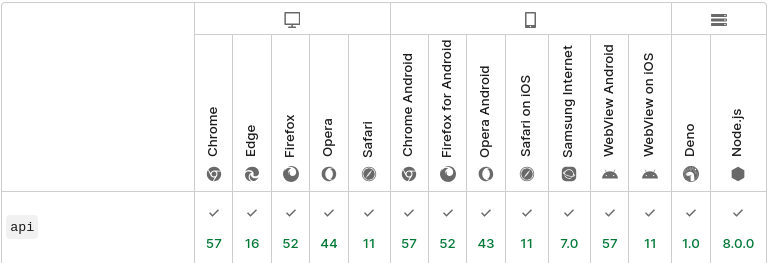
\includegraphics[width=0.95\textwidth]{gfx/figures/webassembly-browsercompability.png}
  \caption{Browser Compatibility: WebAssembly \cite{methodology:wasmdocu}}
  \label{fig:methodology:wasm}
\end{figure}
~\\
\autoref{fig:methodology:wasm} displays the browser compatibility of WebAssembly with multiple major browsers \cite{methodology:wasmdocu}. The check mark indicates WebAssembly support and the green number below marks the version since WebAssembly support was implemented. All browsers are sorted by desktop and mobile version. 

\subsubsection{emscriptren for C and C++}
\label{subsec:methodology:wasm:cpp}
The toolchain, used in this work, to compile C or C++ code into the WebAssembly binary format is emscripten. The team of emscripten already focused on the compilation of C and C++ code to \emph{asm.js} - a predecessor of WebAssembly - in the past \cite{methodology:emcc}. This compiler infrastructure has evolved to target the WebAssembly format, enabling the execution of native C/C++ applications in web browsers. Furthermore, emscripten provides the necessary JavaScript glue code to initialize the WebAssembly environment according to the compiled source code \cite{methodology:emcc}.

\subsubsection{Go}
\label{subsec:methodology:wasm:go}
The standard Go compiler inherently provides a option to directly target the WebAssembly format during the compilation process \cite{methodology:go}. This was utilized to support Go applications in WebArgo. Unlike emscripten, this compilation to WebAssembly is not producing a specific JavaScript glue code file for each Go application, however Go provides a general JavaScript glue code file suitable for all generated WebAssembly binaries \cite{methodology:go}. The files size of this general Go JavaScript glue code is surprisingly small compared to the JavaScript glue code generated by emscripten.

\subsubsection{Pyodie for Python}
\label{subsec:methodology:wasm:python}
Pyodide is described to be a port from CPython to WebAssembly/Emscripten \cite{methodology:pyodie}. It is a JavaScript library that provides a robust foreign function interface to compile python code to WebAssembly and execute it inside the browser environment \cite{methodology:pyodie}. Additionally it enables the installation and execution of Python packages inside the browser using micropip \cite{methodology:pyodie}. Also Pyodide promises, that the executed Python code has full access to the Web \ac{API}s \cite{methodology:pyodie}, which is not an default feature of emscripten or Go.

Unfortunatly, Pyodide performed relatively slow compared to emscripten or Go during the testing of this work. \autoref{sec:evaluation:languages} further investigates the performance of these WebAssembly environments. 

\subsection{WebSockets}
\label{sec:methodology:websockets}
WebSockets play a crucial role for the communication infrastructure of WebArgo. Different from standard \ac{HTTP} requests enable WebSockets a faster, bidirectional and full-duplex communication between clients and servers \cite{methodology:websockets1, methodology:websockets3, methodology:websockets2}. Unlike traditional \ac{HTTP} request-response patterns, WebSocket are establishing a persistent connections between client and server \cite{methodology:websockets3}, allowing real-time data transmission in both directions with minimal overhead after the initial handshake \cite{methodology:websockets3}. This protocol utilizes the ws:// or wss:// (secure) URI scheme and efficiently handles scenarios requiring live updates such as financial trading platforms, multiplayer games, or chat applications, with significantly reduced latency compared to polling mechanisms.

The real-time capability is leveraged for efficient task distribution, progress monitoring, and result collection in the implementation of the WebArgo platform. Additionally, is the bidirectional and full-duplex communication model extremely useful to handle the transmission of task and results between the backend and workers. This replaces inefficient polling strategies and therefore enhances the performance of the communication process between backend and workers.
\\~\\
\autoref{fig:methodology:websocket} displays the browser compatibility of WebSocket with multiple major browsers \cite{methodology:websockets1}. The check mark indicates WebSocket support and the green number below marks the version since WebSocket support was implemented. All browsers are sorted by desktop and mobile version.
\begin{figure}[htbp]
  \centering
  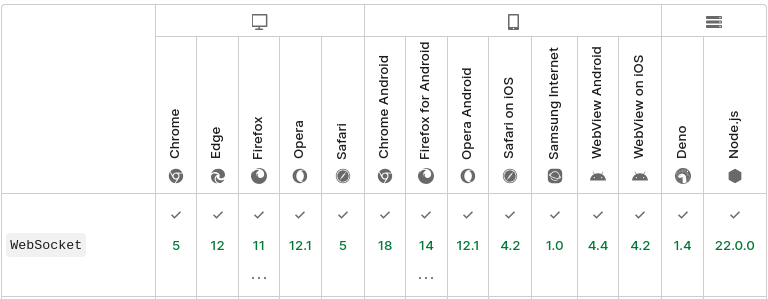
\includegraphics[width=0.95\textwidth]{gfx/figures/websocket-browsercompability.png}
  \caption{Browser Compatibility: WebSocket \cite{methodology:websockets1}}
  \label{fig:methodology:websocket}
\end{figure}

\subsubsection{Socket.IO}
Socket.IO \cite{methodology:websockets2} is a popular JavaScript library that implements the usage of WebSockets on both the server and client side. NestJS \cite{methodology:nestjs}, the selected framework to implement the backend, has an inherent support of Socket.IO, using its concept of so called \emph{Gateways} \cite{methodology:nestjs}. Therefore the Socket.IO libary was selected to implement WebSocket inside the WebArgo platform.

\subsection{WebWorker}
\label{sec:methodology:webworker}
WebWorkers can be accessed through a specific JavaScript \ac{API}, enabling concurrent execution of scripts in background threads separate from the main browser UI thread \cite{methodology:webworkers}. These WebWorkers operate in an isolated context, communicating with the main thread through a message-passing interface, and therefore cannot directly access the \acs{HTML} \acs{DOM} of the web page \cite{methodology:webworkers}. 

This implementation of parallel processing through WebWorkers prevents the computationally intensive WebAssembly execution from blocking the user interface of a worker. This enables the worker to monitor the currently executed task and prevents an unpleasent user experience caused by an unexpectatly frozen screen. Furthermore, the WebWorker \ac{API} allows to create multiple WebWorkers in parallel. This feature could be used in the future to implement a browser based multi-threading solution for WebArgo.
\\~\\
\autoref{fig:methodology:webworker} displays the browser compatibility of WebWorker with multiple major browsers \cite{methodology:webworkers}. The check mark indicates WebWorker support and the green number below marks the version since WebWorker support was implemented. All browsers are sorted by desktop and mobile version.
\newpage
\begin{figure}[htbp]
  \centering
  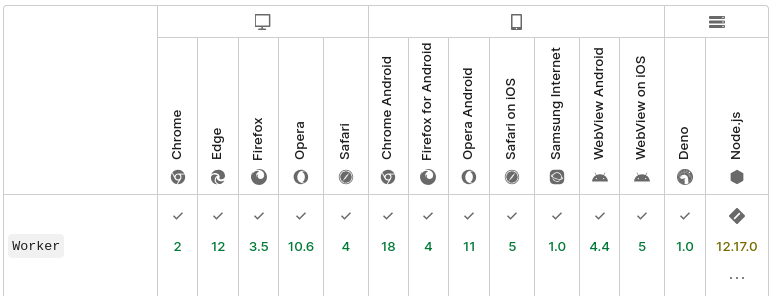
\includegraphics[width=0.95\textwidth]{gfx/figures/webworker-browsercompability.png}
  \caption{Browser Compatibility: WebWorker \cite{methodology:webworkers}}
  \label{fig:methodology:webworker}
\end{figure}

\section{Benchmark: Visualizing the Mandelbrot set}
\label{sec:methodology:benchmark}
To benchmark the platform's performance, a computationally intensive job is implemented and executed across multiple connected workers. The total execution time is compared to the execution time of the same job on a single machine with native source code. The visualization of the Mandelbrot set represents all characteristics previously described in section \ref{sec:concept:theory}, making it suitable as a job for this benchmark.
\begin{figure}[htbp]
  \centering
  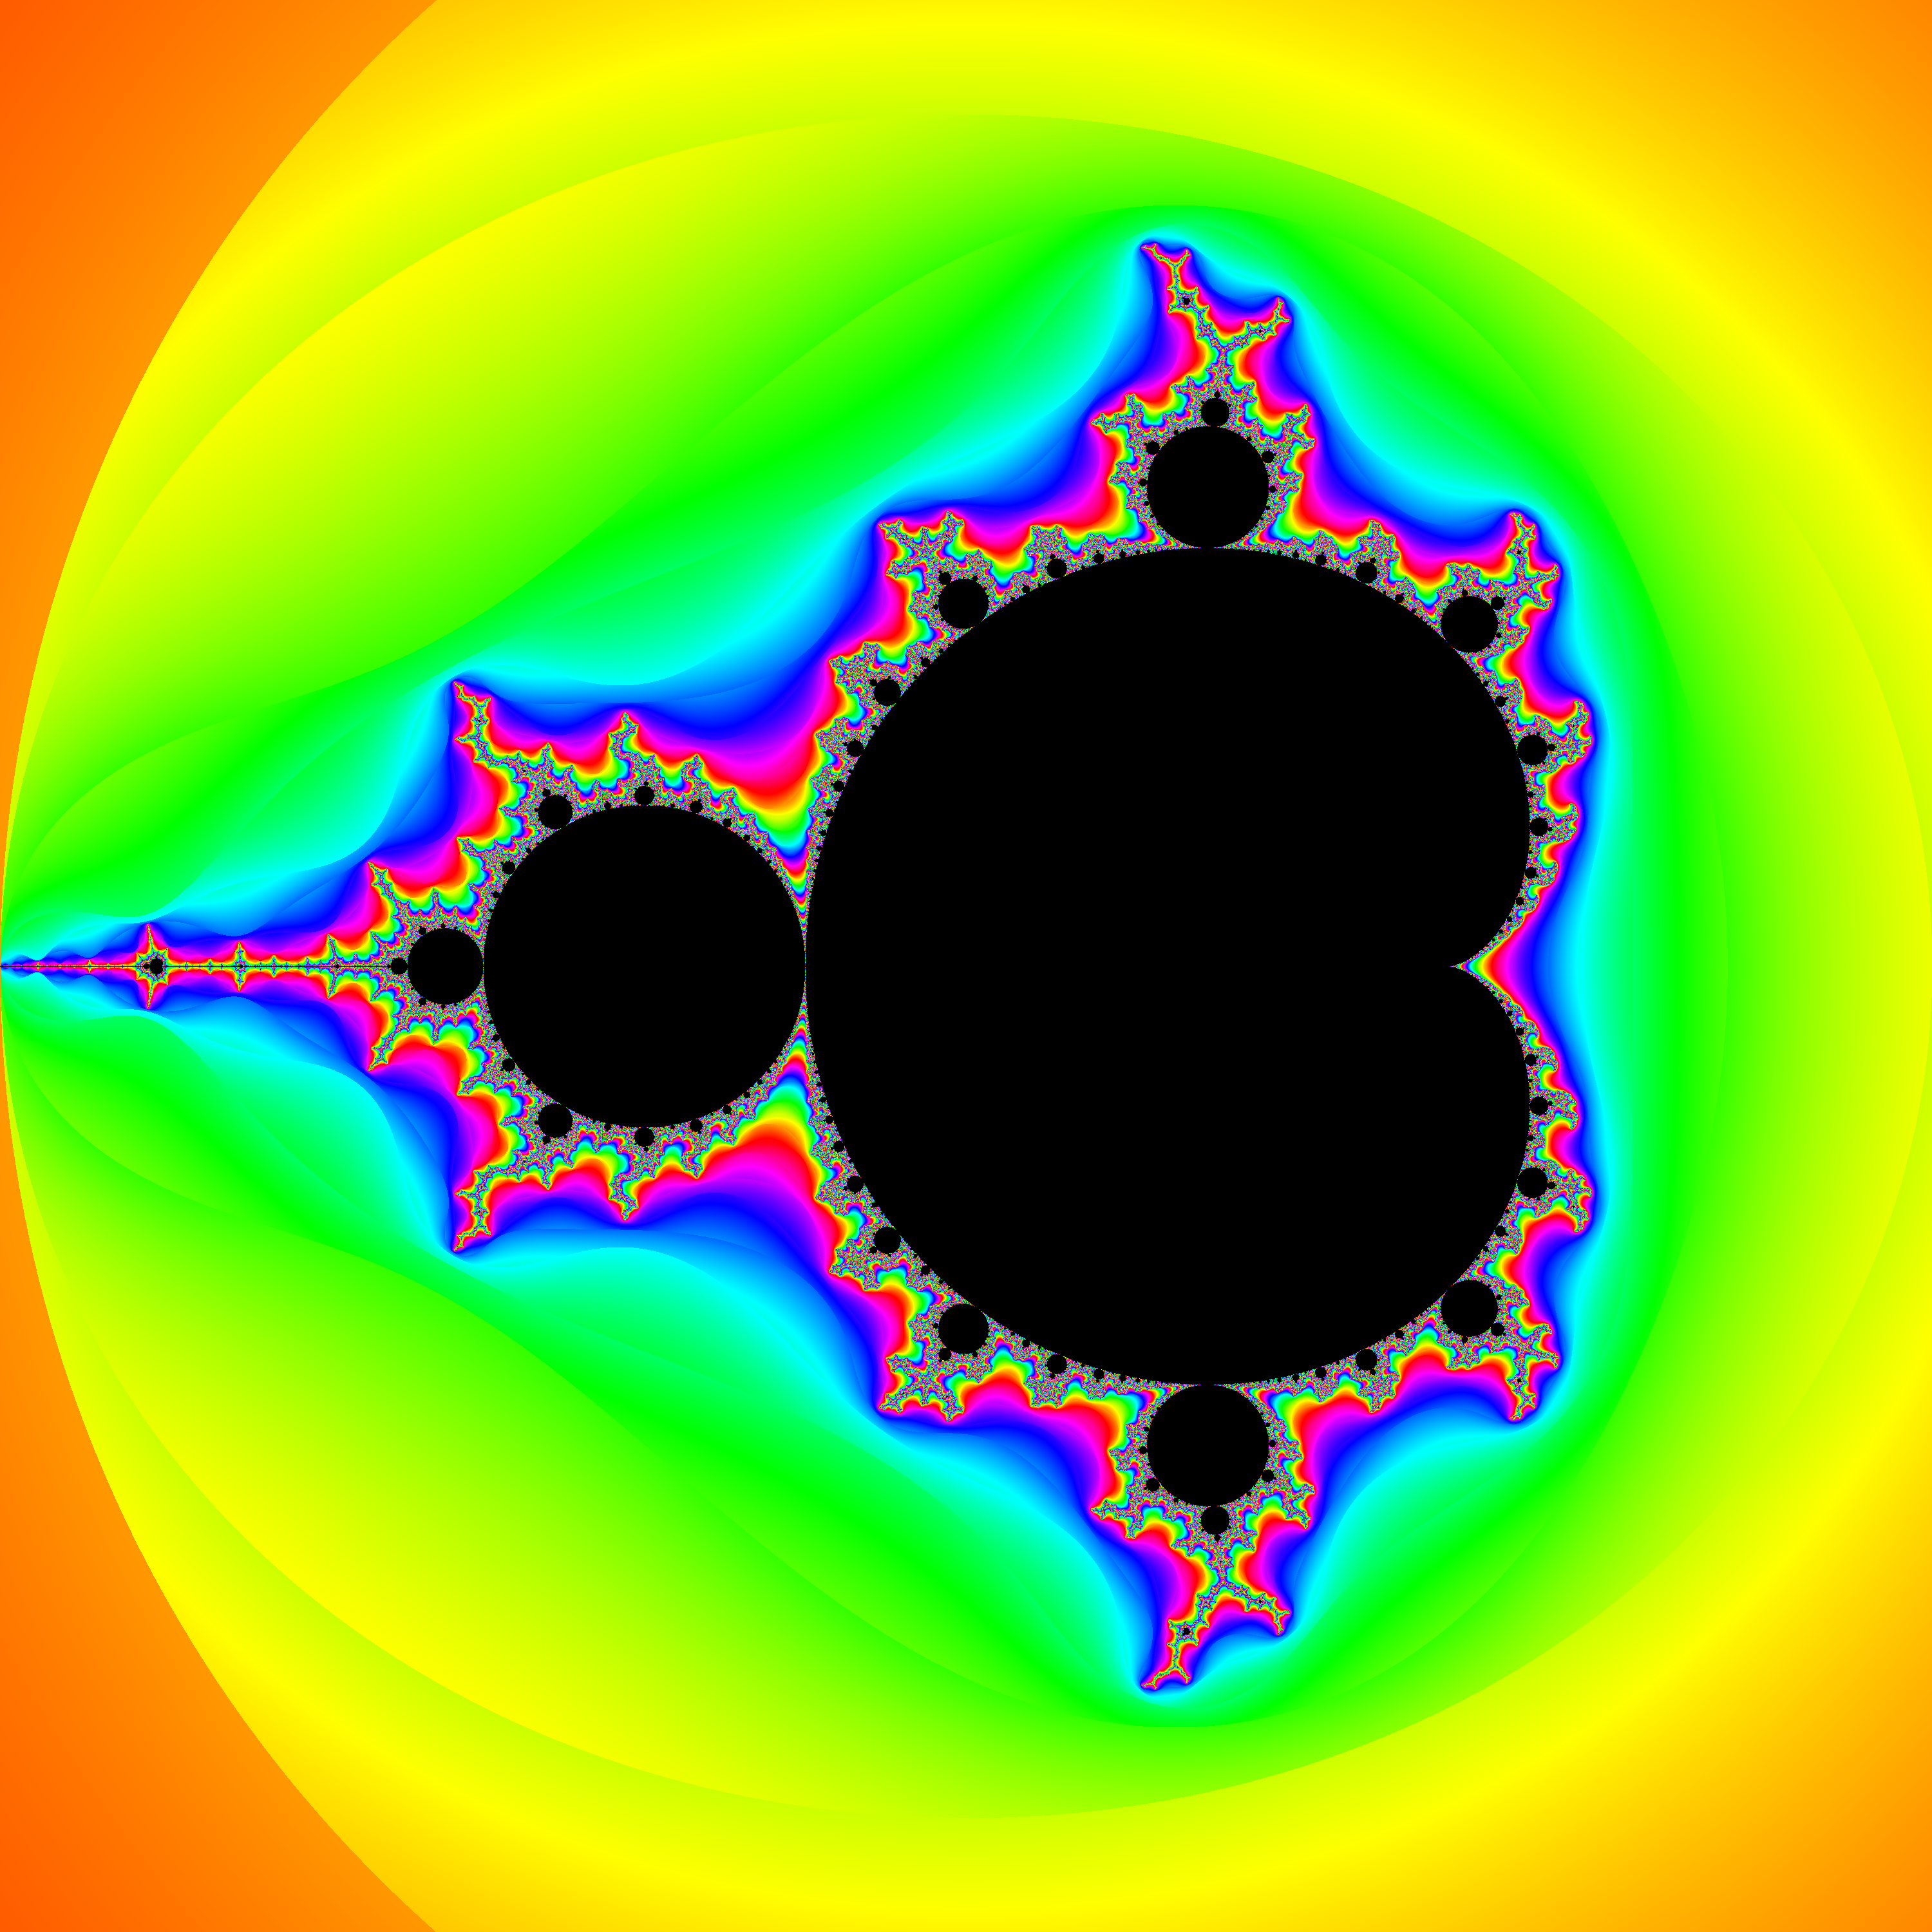
\includegraphics[width=0.75\textwidth]{gfx/figures/mandelbrot.png}
  \caption{Mandelbrot Set (Generated with Code in \autoref{app:code:mandelbrot1})}
  \label{fig:methodology:mandelbrot}
\end{figure}
~\\
The Mandelbrot set is a famous subset of the complex numbers $\mathbb{C}$. \autoref{fig:methodology:mandelbrot} displays a coloriesed visualization of the set in the plane of complex numbers. To determine if a complex number $c$ is part of the Mandelbrot set, $c$ is applied to the function (\ref{equ:mandelbrot}) with $z_{0}=0$.
\begin{equation}
  z_{n+1} = z_{n}^2 + c
  \label{equ:mandelbrot}
\end{equation}
If the value of $z_{n+1}$ does not diverge over $n$ iterations, $c$ belongs to the Mandelbrot set. In \autoref{fig:methodology:mandelbrot}, all complex numbers $c$, for wich $z_{n+1}$ remains bounded over $n$ iterations are colored black. All other $c$ are colored based on the number of iterations required for $z_{n+1}$ to diverge, with the color spectrum ranging from red (low iteration count) over to blue (high iteration count) indicating increasing iteration counts.

The calculation and visualization of the Mandelbrot set can be partitioned into multiple tasks. Each task executes the same source code but with different input parameters, which define a unique two-dimensional area in the complex plane. These tasks can be executed in parallel due to the independence of calculations between different areas. The implementation for this benchmark is provided in \autoref{ch:appendix}. The source code for the native Go variant can be found in \autoref{app:code:mandelbrot1} and its Go-to-WebAssembly counterpart in \autoref{app:code:mandelbrot2}.